\chapter{Related Work} 
\label{Chapter3} 
\lhead{Chapter 3. \emph{Related Work}} 

\section{Native Client Acceleration Modules (NaClAM)} % (fold)
\label{sec:naclam}

In October 2012, John McCutchan at Google came up with the idea of using Native Client as a way to get native performance inside a normal JavaScript web application. He called it ``Native Client Acceleration Modules (NaClAM)'', with a slogan ``\emph{90\% Web App. Native Performance Where You Need It}''.

NaClAM is essentially a simple event-based RPC framework that allowed sending and receiving JavaScript objects as well as binary data. The RPC framework worked by using \emph{event listeners} and \emph{handlers} on both the JavaScript hand C++ ends. 

On the JavaScript side, a library called NaClAM.js was provided, which allowed developers to attach listeners to a particular module using the \lstinline{addEventListener(type,handler)} method. To send requests to the C++, the \lstinline{dispatchEvent} method is used. On the C++ side, messages are handled inside one overridden method called \lstinline{NaClAMModuleHandleMessage}. Here, checks are performed on the message received, and the appropriate method is called. Listing \ref{code_naclam_handle_message} shows an example of this. 

\lstset{language=C++,caption={NaClAM C++ message handler},label=code_naclam_handle_message}
\begin{code}
void NaClAMModuleHandleMessage(const NaClAMMessage& message) {
  if (message.cmdString.compare("floatsum") == 0) {
    handleFloatSum(message);
  } else if (message.cmdString.compare("addfloatarrays") == 0) {
    handleAddFloats(message);
  } else {
    NaClAMPrintf("Got message I don't understand");
  }
}
\end{code}

\subsection{Message Format} % (fold)
\label{sub:naclam_message_format}
\begin{figure}
	\centering
	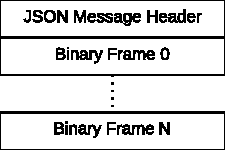
\includegraphics[width=0.3\textwidth]{naclam-msg-format.pdf} 
	\caption{A NaClAM message including binary frames}
	\label{fig:naclam_msg_format}
\end{figure}

At the message passing level, NaClAM uses JavaScript/C++ strings to transport messages. These messages hold information about the message such as the command string (like ``\lstinline{floatsum}'' in listing \ref{code_naclam_handle_message}). The strings are constructed using the jsoncpp library. 

Crucially, however, they also tell the framework how many binary \emph{frames} are expected to come after this message. Figure \ref{fig:naclam_msg_format} shows an example of a message containing $N$ frames. A frame is essentially a binary block of data sent by a separate call to \lstinline{PostMessage}. The receiver collects all the frames before triggering the event handler.

% subsection naclam_message_format (end)

\subsection{Advantages and Disadvantages} % (fold)
\label{sub:naclam_advantages_and_disadvantages}
NaClAM modules have the benefit of being simple and fast. There is a good distinction between the message information stored in the header and the message data stored as binary inside the frames. This allows developers to use the message header to implement event logic, while using the frames to transfer actual data. It also means that because the data is binary and almost no marshalling happens, the transfer speed is very fast, since binary data is \emph{shared} between JavaScript and C++.

However, there are a few issues with using NaClAM modules. The first is a lack of overall, high-level structure. The developer has to be aware and understand exactly what the framework is doing behind the scenes to write their application, which adds more burden on the developer, especially since almost no documentation is provided. The second issue is how the message header types are implemented. Although the framework allows sending application data in binary frames, the header information is sent as JSON, and is manipulated by the jsoncpp library - so another library the developer needs to get used to. Importantly, this means the developer needs to unpack and pack the data they are sending in the header section by themselves by using the jsoncpp library. Another issue is how the framework does not use a callback approach to asynchronous remote procedure calls. In other words, to `return' a value from a C++ function back to JavaScript, a \emph{different} event needs to be triggered from the C++, and handled by the JavaScript library. In other words, two different events need to be managed in both C++ and JavaScript for only one RPC call which returns data. If there are many functions like this, the developer needs to manage several different events, which is tedious. Finally, although the framework has been demoed and gained a lot of popularity, it still seems to not be well tested, as no unit tests exist for either the C++ or JavaScript implementations have been written. This makes it feel like an experimental project, rather than a full, well supported framework. 

Despite these issues, the Native Calls project was heavily influenced and inspired by the overall idea of the NaClAM project, especially its use cases and scenarios.
% subsection naclam_advantages_and_disadvantages (end)

% section naclam (end)

\section{Node.js C++ Bindings} % (fold)
\label{sec:node_js_c_bindings}
TODO: node.js C++ bindings. Mention:
\begin{itemize}
	\item Idea, example
	\item Typical implementation example
	\item Advantages, disadvantages
\end{itemize}
% section node_js_c_bindings (end)



\section{Apache Thrift: Cross-language services} % (fold)
\label{sec:apache_thrift_cross_language_services}
Apache Thrift is a framework that allows cross-language services development. Originally developed at Facebook, it was designed to provide reliable, efficient communication between languages and services. Many languages are supported, including C++, Java, and JavaScript. Thrift provides a cross-platform generator that can generate Thrift client and server pairs, where the client and server can be using different languages. Similar to other RPC frameworks, it uses its own IDL file format, Thrift IDL. The IDL file is used to generate code to support different languages.

An unofficial port for Apache Thrift has been made for Native Client \footnote{\url{https://github.com/ahilss/thrift-nacl}}, however, all of the communication code is still hand coded. The performance of using Thrift for Native Client is unclear, as there is no protocol implemented using PPAPI.

TODO: Better structure this section. Mention:
\begin{itemize}
	\item Idea, example.
	\item Typical implementation example, use cases.
	\item Advantages, disadvantages
\end{itemize}

% section apache_thrift_cross_language_services (end)


\section{JSON-RPC Implementations} % (fold)

TODO: Better structure this section. Include:
\begin{itemize}
	\item What they are, general design of these frameworks.
	\item Example: pmrpc (+advantages, disadvantages)
	\item General: Advantages, disadvantages
\end{itemize}

\label{sec:json_rpc_implementations}
Many JSON-RPC implementations for several languages exist\footnote{\url{http://en.wikipedia.org/wiki/JSON-RPC}}, including C++\footnote{\url{http://jsonrpc-cpp.sourceforge.net/}} and JavaScript\footnote{\url{https://github.com/gimmi/jsonrpcjs}}. However, none have been implemented for Native Client and using the PPAPI API.

\subsection{pmrpc: Inter-window JavaScript RPC using postMessage} % (fold)
\label{sub:pmrpc_json_rpc_using_postmessage}
pmrpc is an open source library available on GitHub \footnote{\url{https://github.com/izuzak/pmrpc}} which aims to simplify cross-window communication by using postMessage. It shows the simplicity of remote procedure calls using JSON-RPC but only supports browser-based JavaScript. Native Client C++ or any other language or transport is not supported.
% subsection pmrpc_json_rpc_using_postmessage (end)

% section json_rpc_implementations (end)